%----------------------------------------------------------------------------
\chapter{Application expectations}\label{Ch1}
%----------------------------------------------------------------------------
In this section I will shortly discuss the chosen problem, so that the reader can understand the main goal and context of the following chapters. We will take a look at the user story, then break it down to use cases. At the second part of the chapter we will compose three user flows based on them.
%----------------------------------------------------------------------------
\section{User Story}
%----------------------------------------------------------------------------

Under real life circumstances the developer gets a vague and not at all professional description of what the job would be. I wanted to simulate this because it would give us a compact description of the problem. The user story I created for myself in this instance reads as follows: 

 \emph{
 	We need an application where restaurants can be registered, upload their offers and other useful data like opening hours. Guests can also log in and order food for takeaway or dine in. In the second case let them choose a table at the restaurant. They should also provide information about when they want to take it or eat the dish, so they can be served minutes after arrival. Guests pay in advance right after order, so there will be fewer cases of unclaimed orders. Also they don't have to wait for payment on site. Guests can give feedback on their experience.
 } 

For simplicity's sake from now on I will call this app \emph{Allegro}.

%----------------------------------------------------------------------------
\section{Use Cases}
%----------------------------------------------------------------------------
 As a next step, I defined the use cases based on the user story and created the following use case diagram (Figure \figref{UseCaseDiagram}). I will give a short summary below. 
 
We have three potential Actors: 

\begin{itemize}
	\item \verb+Anonymous Users+,
	\item \verb+Guests+, who are logged in users without a restaurant connected to them,
	\item \verb+Restaurants+, who are logged in users with a restaurant.
\end{itemize}

 \begin{figure}[!ht]
	\centering
	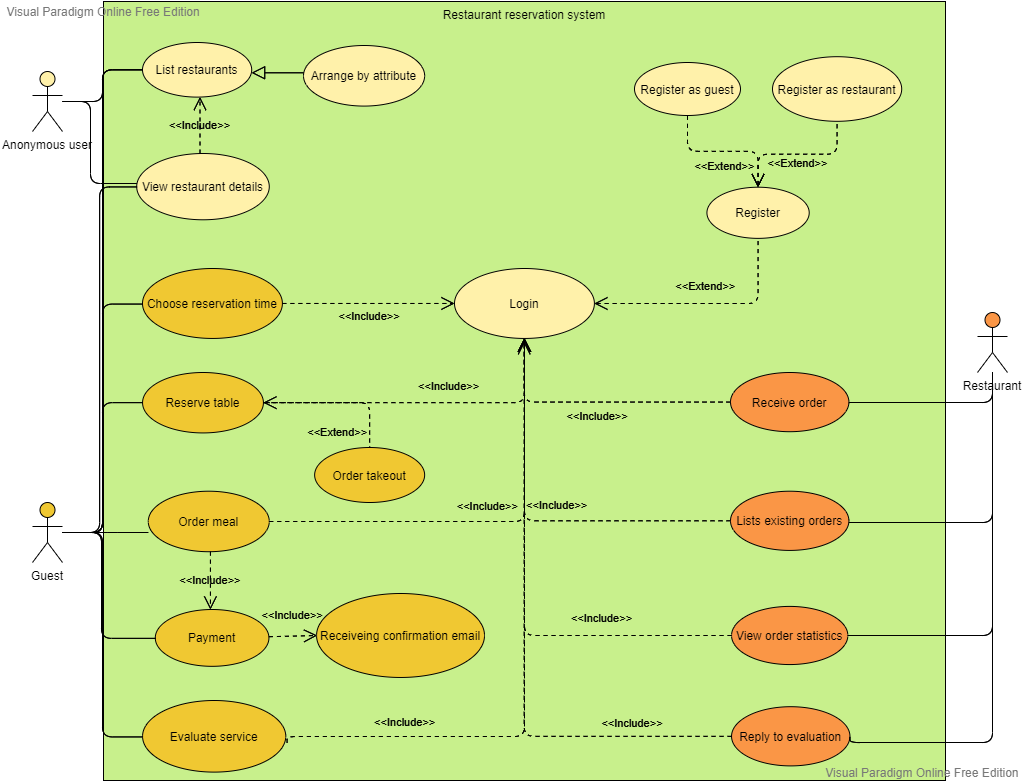
\includegraphics[width=150mm, keepaspectratio]{figures/UseCaseDiagram}
	\caption{Use Case Diagram} 
	\label{fig:UseCaseDiagram}
\end{figure}

\verb+Anonymous Users+ have the options to list existing restaurants, view them one by one in a detailed view, log in if they already have an account or create a guest or restaurant account. 

Someone with a \verb+Guest+ account can walk through the food ordering process which includes reserving table at a given restaurant for a given date and time, ordering meal and paying for these. They can also evaluate the restaurant they ordered at.

\verb+Restaurants+ will have the ability to receive orders, list them, view their statistics and write a reply to guest evaluations.

The full list of the created use cases can be found in the Appendix under \ref{usecases}.

%----------------------------------------------------------------------------
\section{User Flows}
%----------------------------------------------------------------------------

After the use cases were finished, I could move to figuring out how the users were expected to interact with the application. As we see on the use case diagram, I defined three roles. Here I'll give a short description of each.
%----------------------------------------------------------------------------
\subsection{Anonymous User}\label{AnonUserflow}
%----------------------------------------------------------------------------
 Based on the use cases, I thought a restaurant list would be a good entry point for the users. From there it should be an option to choose a specific restaurant and navigate to its details page. The anonymous user's use cases are, in this way, properly handled, so at this point there should be a login option which diverges to the guest and the restaurant user flow. See a graphic explanation at Figure \figref{UIsAnon}
\begin{figure}[!ht]
	\centering
	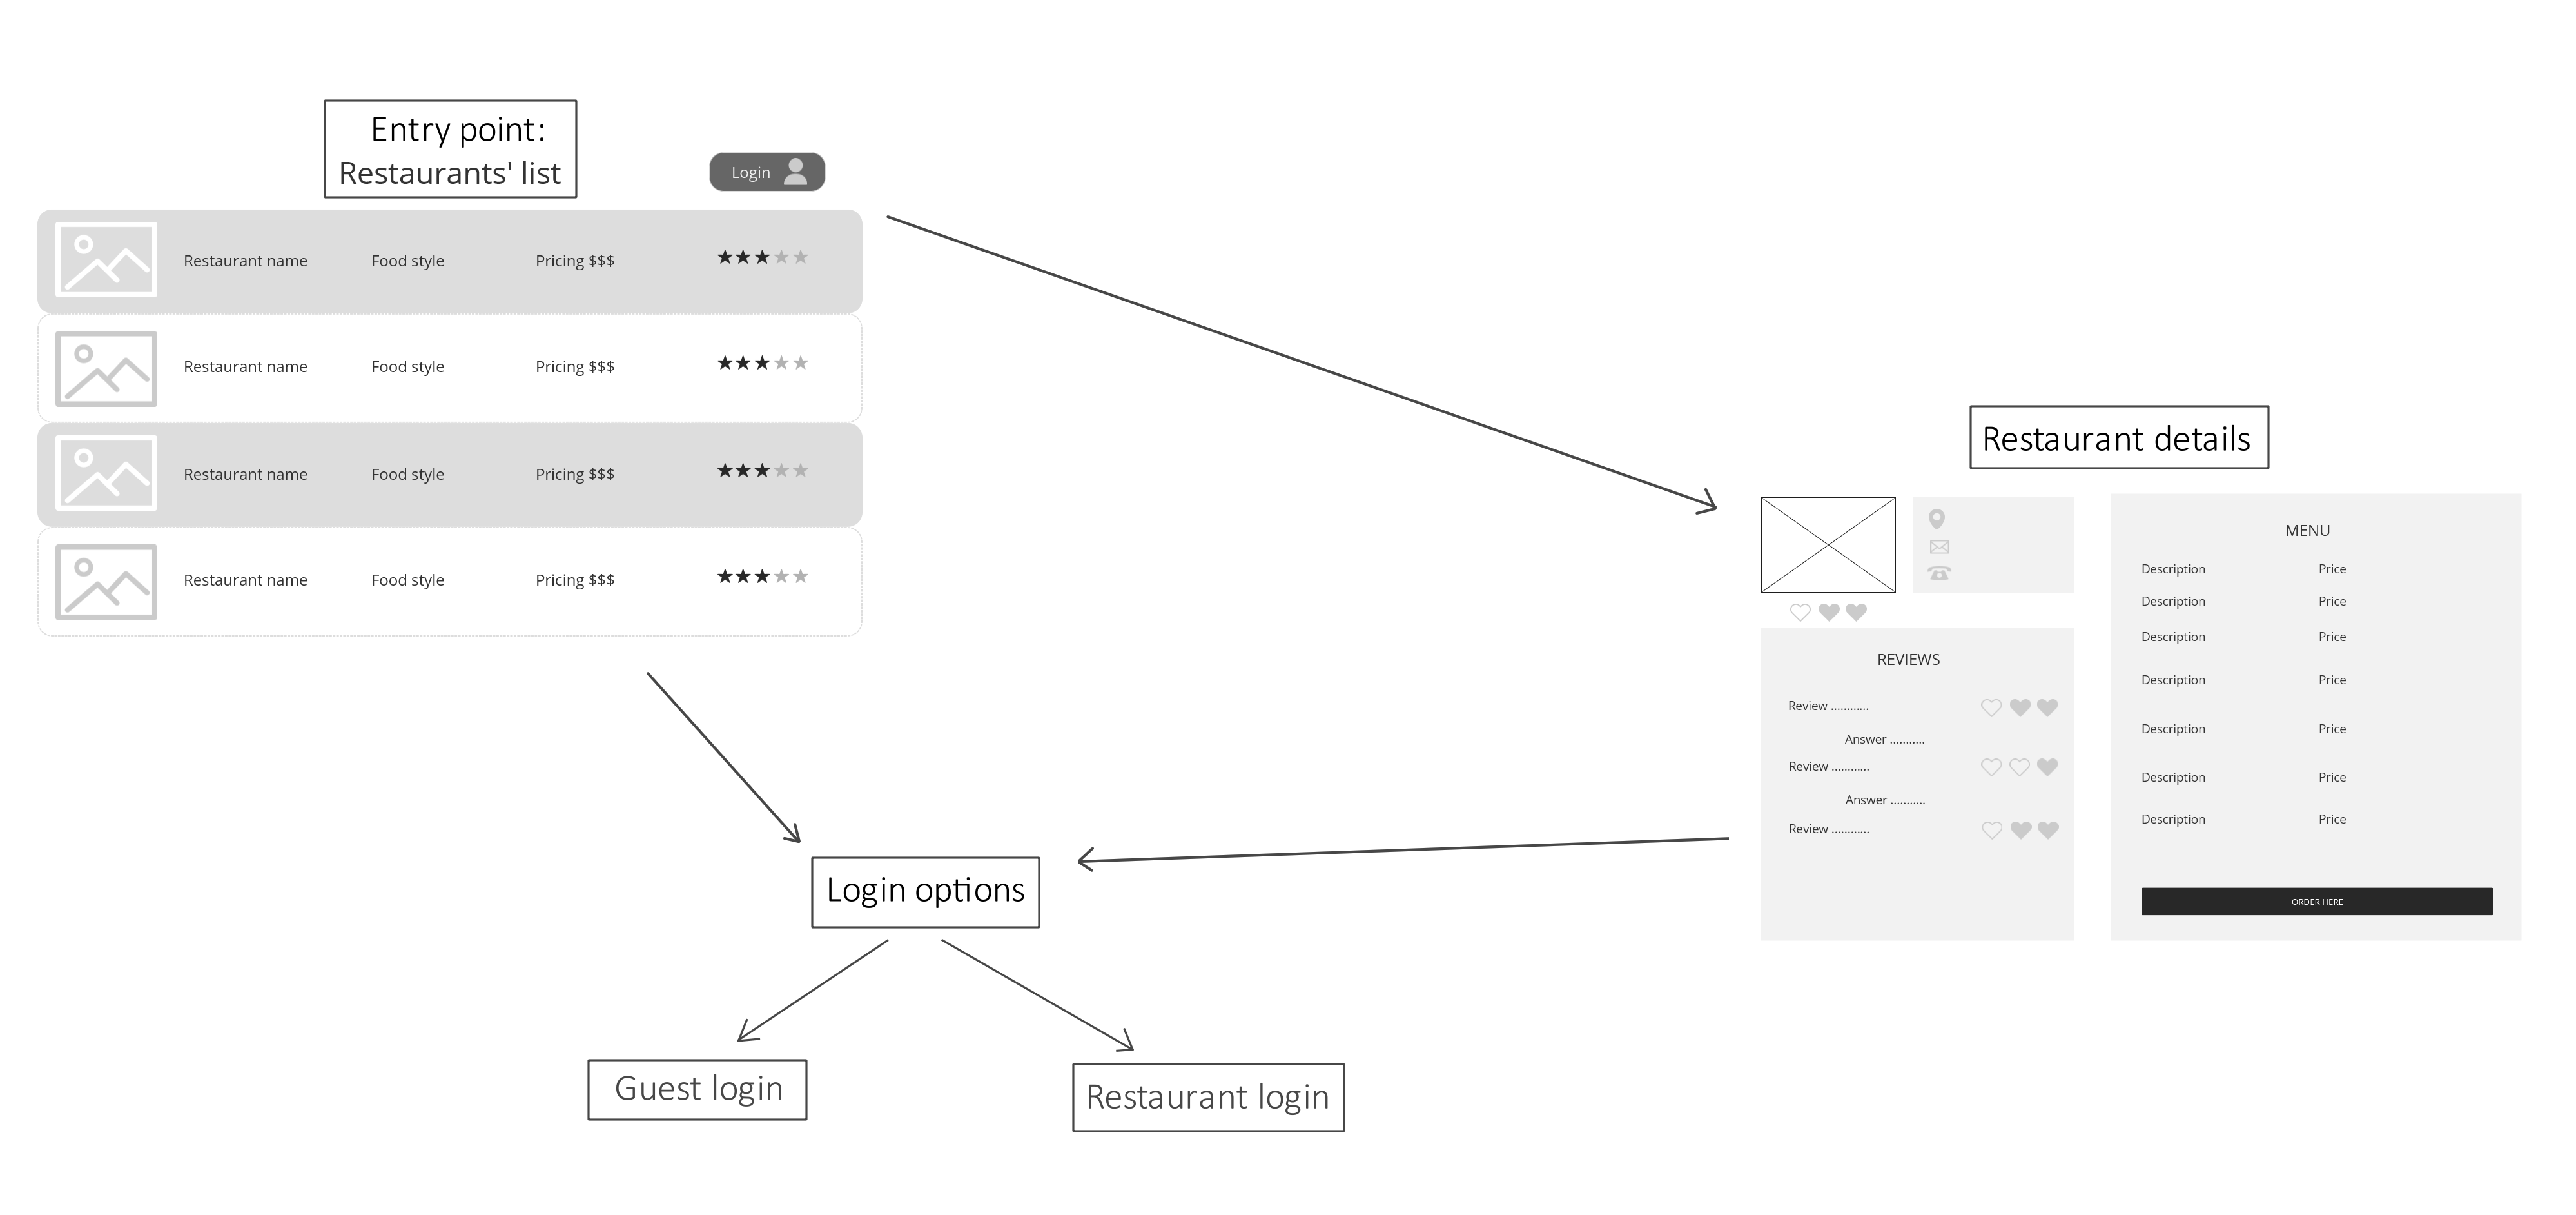
\includegraphics[width=150mm, keepaspectratio]{figures/UIsAnon.png}
	\caption{Anonymous user's user flow} 
	\label{fig:UIsAnon}
\end{figure}
%----------------------------------------------------------------------------
\subsection{Guest}\label{GuestUserflow}
%----------------------------------------------------------------------------
At the login page there should be an option to sign in or register as a guest or to do the same as a restaurant owner. Following the use case diagram, a guest can choose a restaurant to order from, so after signing in he should start his journey at the restaurants' list page then to the details page and then navigate to an order site provided he is, indeed, authenticated. Alternatively, in case we allow to start the order process as an anonymous user, the user should be prompted to log in, then redirected to the chosen restaurant's order page. Here he should be able to book a table or order takeaway and save the date and time. Next, he can navigate to the menu and pick the wished dishes. Afterwards, the order details can be checked and modified and finally the payment can be done. Here we would like to send e-mails to the guest about the successful payment and the order details. Finally, the guest can send a feedback about his experiences. See Figure \figref{UIsGuest}
\begin{figure}[!ht]
	\centering
	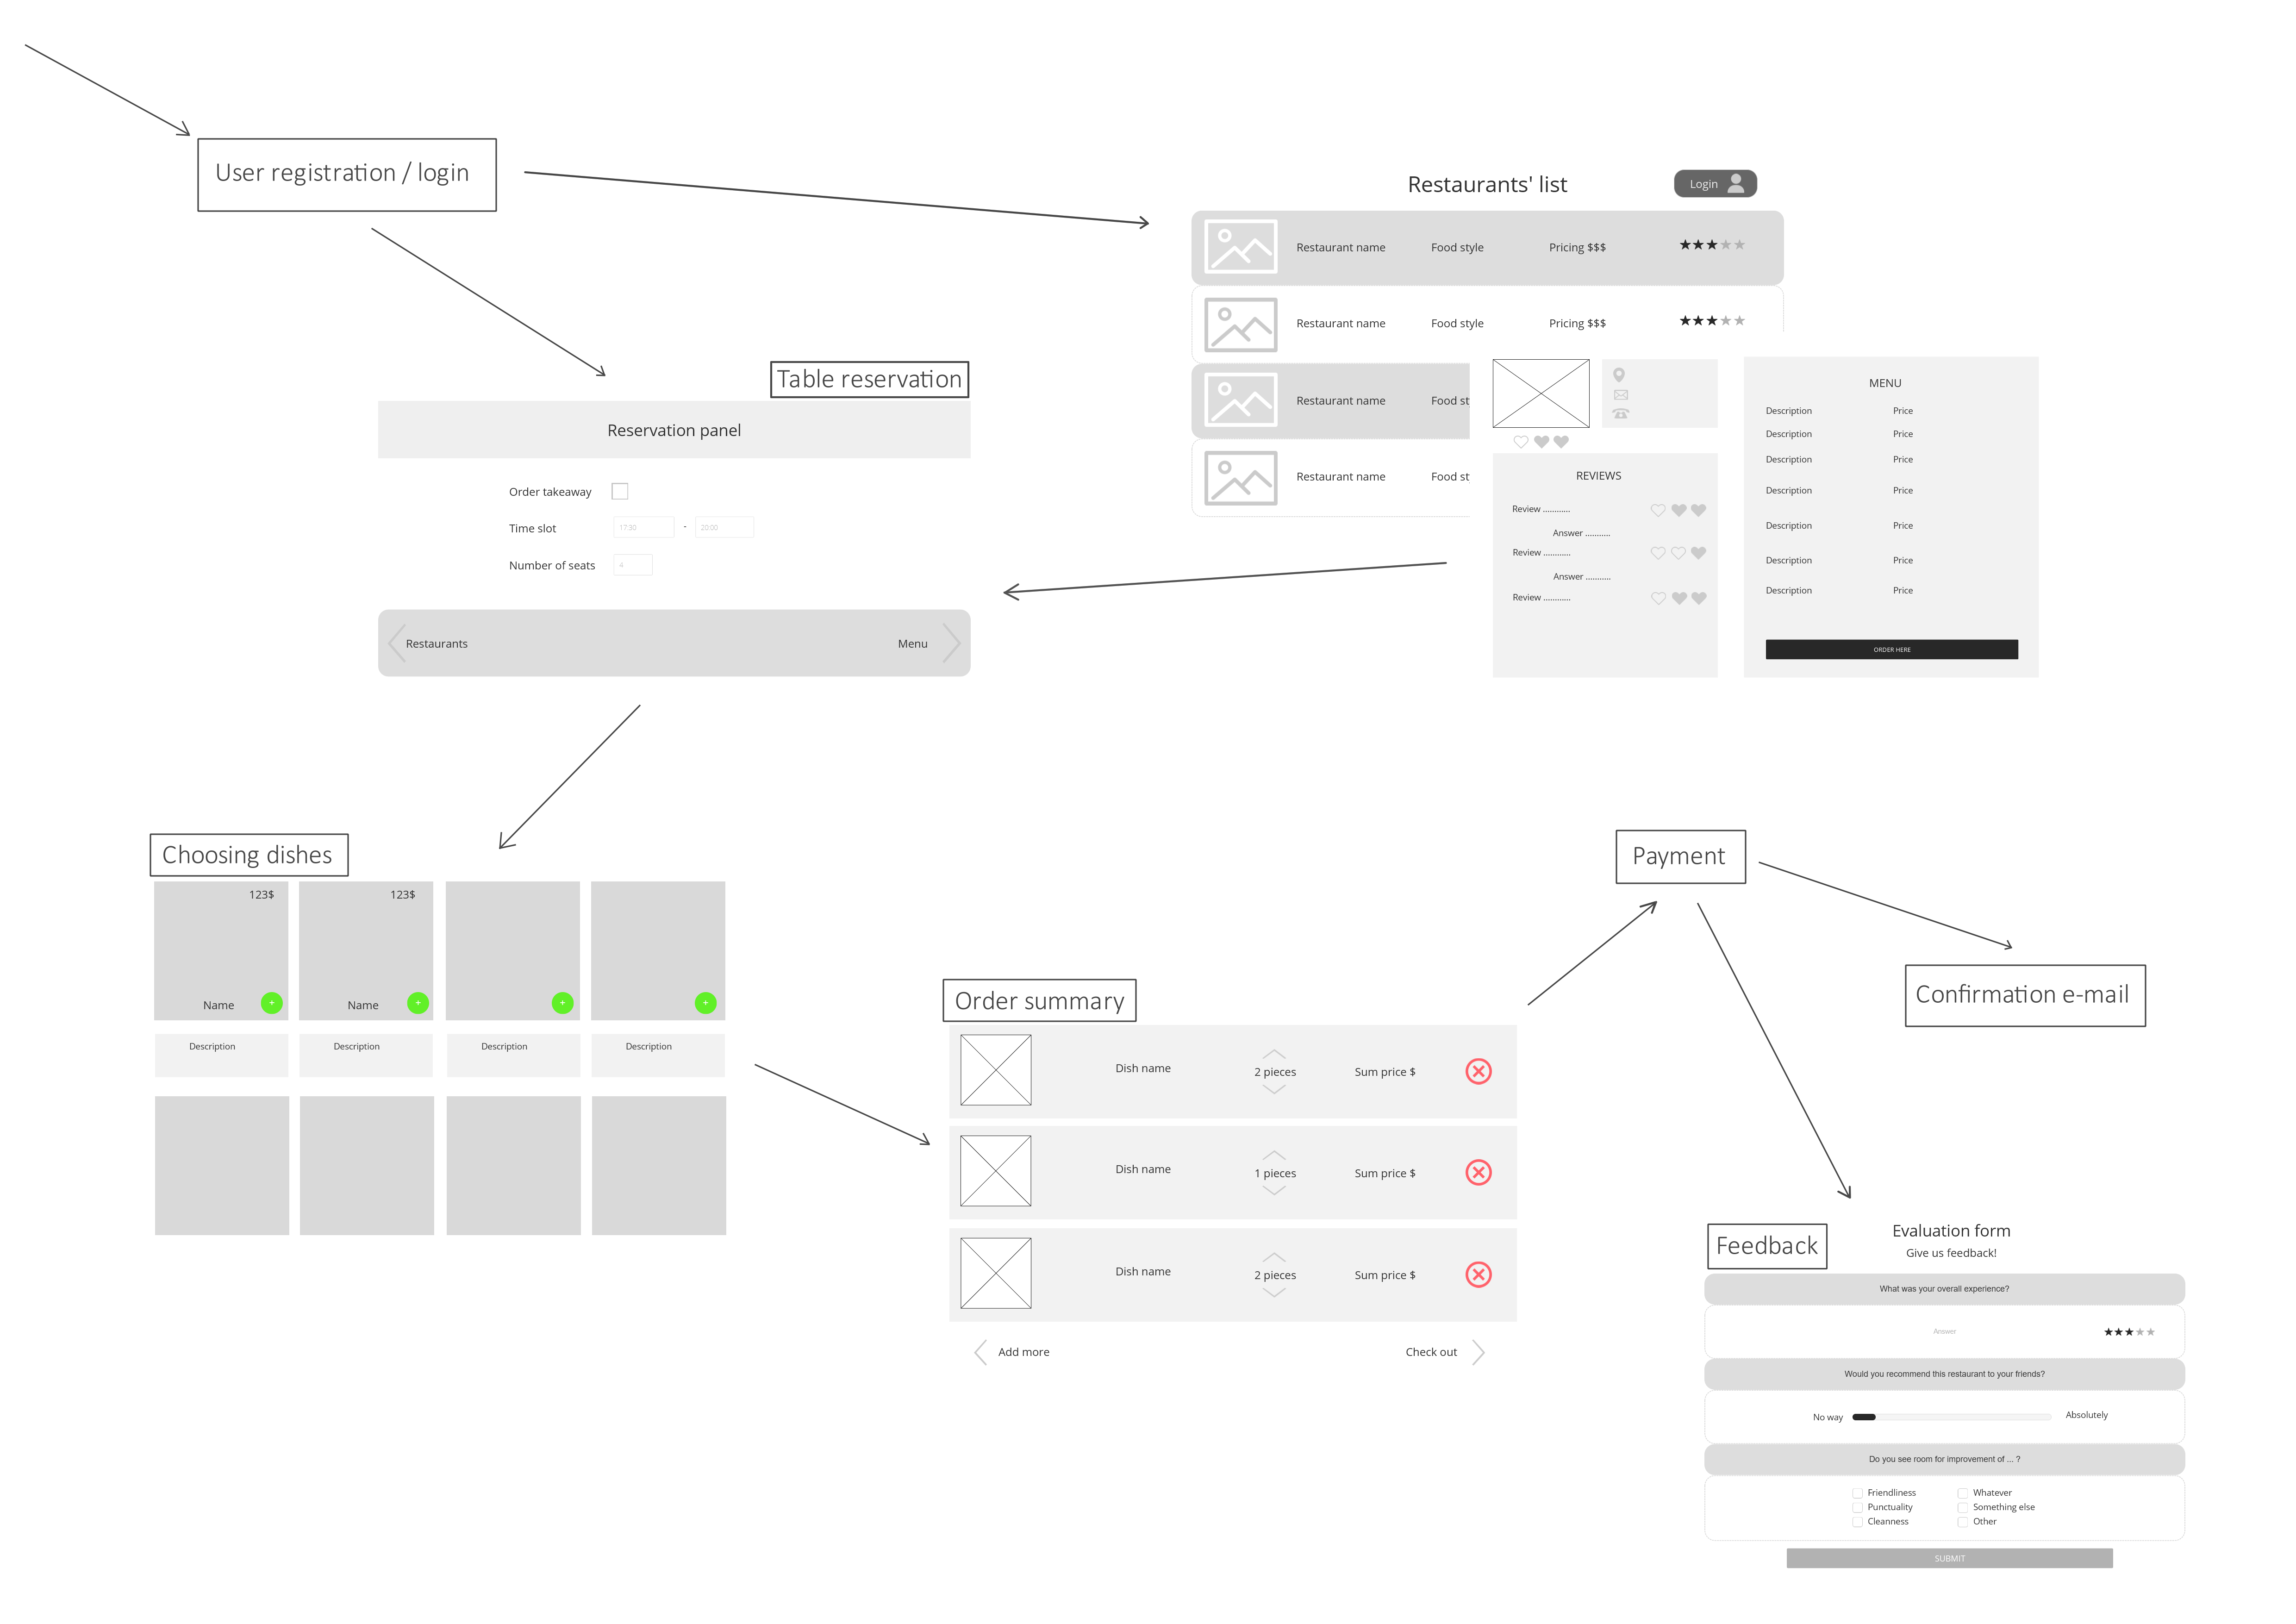
\includegraphics[width=150mm, keepaspectratio]{figures/UIsGuest.png}
	\caption{Guest's user flow} 
	\label{fig:UIsGuest}
\end{figure}
%----------------------------------------------------------------------------
\subsection{Restaurant}\label{RestaurantUserflow}
%----------------------------------------------------------------------------
If one decides to create a new restaurant, he has to register through three steps. First, the basic data should be collected e.g.\ contact information. Then the restaurant user can add the menu and finally the table information, from which the guests will choose from. If the registration was successful, the restaurant user can log in and will be redirected to a dashboard, where the restaurant's orders and reviews will be displayed. From here he can navigate to data modification pages and can answer to the reviews. See Figure \figref{UIsRestaurant}
\begin{figure}[!ht]
	\centering
	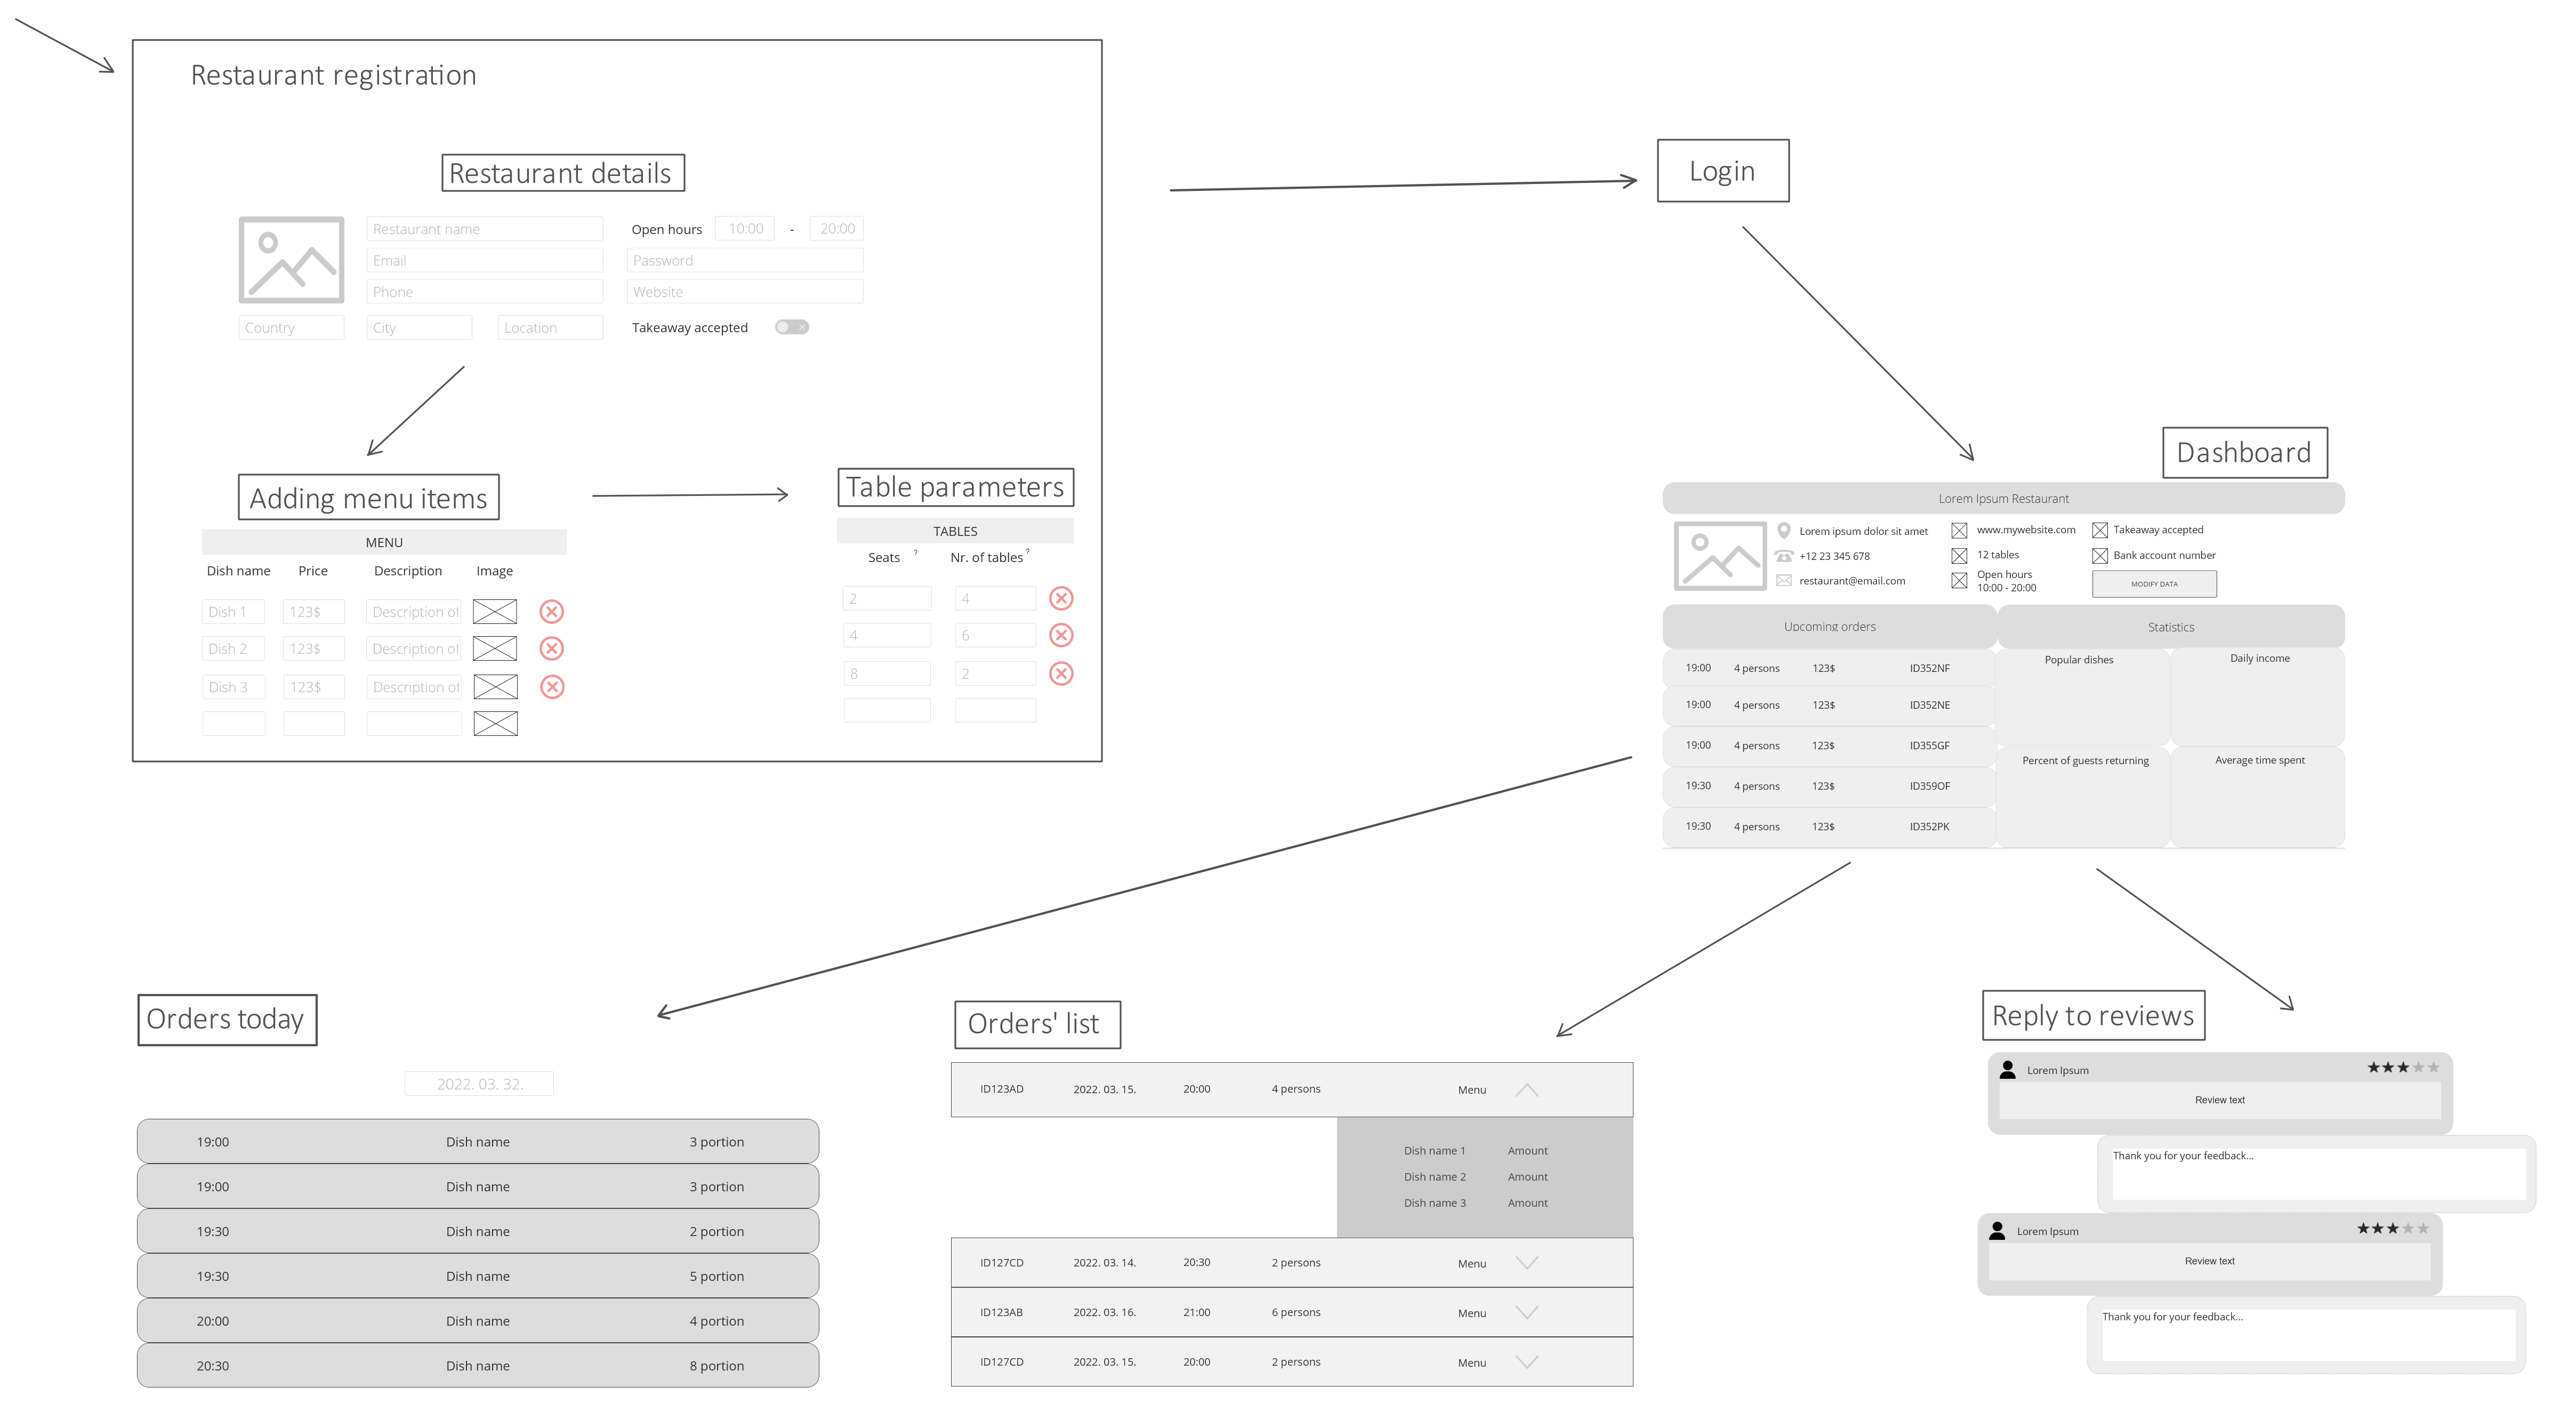
\includegraphics[width=150mm, keepaspectratio]{figures/UIsRestaurant.png}
	\caption{Restaurant's user flow} 
	\label{fig:UIsRestaurant}
\end{figure}